\documentclass[1p]{elsarticle_modified}
%\bibliographystyle{elsarticle-num}

%\usepackage[colorlinks]{hyperref}
%\usepackage{abbrmath_seonhwa} %\Abb, \Ascr, \Acal ,\Abf, \Afrak
\usepackage{amsfonts}
\usepackage{amssymb}
\usepackage{amsmath}
\usepackage{amsthm}
\usepackage{scalefnt}
\usepackage{amsbsy}
\usepackage{kotex}
\usepackage{caption}
\usepackage{subfig}
\usepackage{color}
\usepackage{graphicx}
\usepackage{xcolor} %% white, black, red, green, blue, cyan, magenta, yellow
\usepackage{float}
\usepackage{setspace}
\usepackage{hyperref}

\usepackage{tikz}
\usetikzlibrary{arrows}

\usepackage{multirow}
\usepackage{array} % fixed length table
\usepackage{hhline}

%%%%%%%%%%%%%%%%%%%%%
\makeatletter
\renewcommand*\env@matrix[1][\arraystretch]{%
	\edef\arraystretch{#1}%
	\hskip -\arraycolsep
	\let\@ifnextchar\new@ifnextchar
	\array{*\c@MaxMatrixCols c}}
\makeatother %https://tex.stackexchange.com/questions/14071/how-can-i-increase-the-line-spacing-in-a-matrix
%%%%%%%%%%%%%%%

\usepackage[normalem]{ulem}

\newcommand{\msout}[1]{\ifmmode\text{\sout{\ensuremath{#1}}}\else\sout{#1}\fi}
%SOURCE: \msout is \stkout macro in https://tex.stackexchange.com/questions/20609/strikeout-in-math-mode

\newcommand{\cancel}[1]{
	\ifmmode
	{\color{red}\msout{#1}}
	\else
	{\color{red}\sout{#1}}
	\fi
}

\newcommand{\add}[1]{
	{\color{blue}\uwave{#1}}
}

\newcommand{\replace}[2]{
	\ifmmode
	{\color{red}\msout{#1}}{\color{blue}\uwave{#2}}
	\else
	{\color{red}\sout{#1}}{\color{blue}\uwave{#2}}
	\fi
}

\newcommand{\Sol}{\mathcal{S}} %segment
\newcommand{\D}{D} %diagram
\newcommand{\A}{\mathcal{A}} %arc


%%%%%%%%%%%%%%%%%%%%%%%%%%%%%5 test

\def\sl{\operatorname{\textup{SL}}(2,\Cbb)}
\def\psl{\operatorname{\textup{PSL}}(2,\Cbb)}
\def\quan{\mkern 1mu \triangleright \mkern 1mu}

\theoremstyle{definition}
\newtheorem{thm}{Theorem}[section]
\newtheorem{prop}[thm]{Proposition}
\newtheorem{lem}[thm]{Lemma}
\newtheorem{ques}[thm]{Question}
\newtheorem{cor}[thm]{Corollary}
\newtheorem{defn}[thm]{Definition}
\newtheorem{exam}[thm]{Example}
\newtheorem{rmk}[thm]{Remark}
\newtheorem{alg}[thm]{Algorithm}

\newcommand{\I}{\sqrt{-1}}
\begin{document}

%\begin{frontmatter}
%
%\title{Boundary parabolic representations of knots up to 8 crossings}
%
%%% Group authors per affiliation:
%\author{Yunhi Cho} 
%\address{Department of Mathematics, University of Seoul, Seoul, Korea}
%\ead{yhcho@uos.ac.kr}
%
%
%\author{Seonhwa Kim} %\fnref{s_kim}}
%\address{Center for Geometry and Physics, Institute for Basic Science, Pohang, 37673, Korea}
%\ead{ryeona17@ibs.re.kr}
%
%\author{Hyuk Kim}
%\address{Department of Mathematical Sciences, Seoul National University, Seoul 08826, Korea}
%\ead{hyukkim@snu.ac.kr}
%
%\author{Seokbeom Yoon}
%\address{Department of Mathematical Sciences, Seoul National University, Seoul, 08826,  Korea}
%\ead{sbyoon15@snu.ac.kr}
%
%\begin{abstract}
%We find all boundary parabolic representation of knots up to 8 crossings.
%
%\end{abstract}
%\begin{keyword}
%    \MSC[2010] 57M25 
%\end{keyword}
%
%\end{frontmatter}

%\linenumbers
%\tableofcontents
%
\newcommand\colored[1]{\textcolor{white}{\rule[-0.35ex]{0.8em}{1.4ex}}\kern-0.8em\color{red} #1}%
%\newcommand\colored[1]{\textcolor{white}{ #1}\kern-2.17ex	\textcolor{white}{ #1}\kern-1.81ex	\textcolor{white}{ #1}\kern-2.15ex\color{red}#1	}

{\Large $\underline{12n_{0355}~(K12n_{0355})}$}

\setlength{\tabcolsep}{10pt}
\renewcommand{\arraystretch}{1.6}
\vspace{1cm}\begin{tabular}{m{100pt}>{\centering\arraybackslash}m{274pt}}
\multirow{5}{120pt}{
	\centering
	\includegraphics[width=112pt]{../../../GIT/diagram.site/Diagrams/png/2444_12n_0355.png}\\
\ \ \ A knot diagram\footnotemark}&
\allowdisplaybreaks
\textbf{Linearized knot diagam} \\
\cline{2-2}
 &
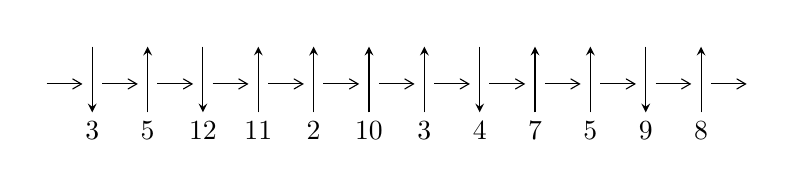
\begin{tikzpicture}[x=20pt, y=17pt]
	% nodes
	\node (C0) at (0, 0) {};
	\node (C1) at (1, 0) {};
	\node (C1U) at (1, +1) {};
	\node (C1D) at (1, -1) {3};

	\node (C2) at (2, 0) {};
	\node (C2U) at (2, +1) {};
	\node (C2D) at (2, -1) {5};

	\node (C3) at (3, 0) {};
	\node (C3U) at (3, +1) {};
	\node (C3D) at (3, -1) {12};

	\node (C4) at (4, 0) {};
	\node (C4U) at (4, +1) {};
	\node (C4D) at (4, -1) {11};

	\node (C5) at (5, 0) {};
	\node (C5U) at (5, +1) {};
	\node (C5D) at (5, -1) {2};

	\node (C6) at (6, 0) {};
	\node (C6U) at (6, +1) {};
	\node (C6D) at (6, -1) {10};

	\node (C7) at (7, 0) {};
	\node (C7U) at (7, +1) {};
	\node (C7D) at (7, -1) {3};

	\node (C8) at (8, 0) {};
	\node (C8U) at (8, +1) {};
	\node (C8D) at (8, -1) {4};

	\node (C9) at (9, 0) {};
	\node (C9U) at (9, +1) {};
	\node (C9D) at (9, -1) {7};

	\node (C10) at (10, 0) {};
	\node (C10U) at (10, +1) {};
	\node (C10D) at (10, -1) {5};

	\node (C11) at (11, 0) {};
	\node (C11U) at (11, +1) {};
	\node (C11D) at (11, -1) {9};

	\node (C12) at (12, 0) {};
	\node (C12U) at (12, +1) {};
	\node (C12D) at (12, -1) {8};
	\node (C13) at (13, 0) {};

	% arrows
	\draw[->,>={angle 60}]
	(C0) edge (C1) (C1) edge (C2) (C2) edge (C3) (C3) edge (C4) (C4) edge (C5) (C5) edge (C6) (C6) edge (C7) (C7) edge (C8) (C8) edge (C9) (C9) edge (C10) (C10) edge (C11) (C11) edge (C12) (C12) edge (C13) ;	\draw[->,>=stealth]
	(C1U) edge (C1D) (C2D) edge (C2U) (C3U) edge (C3D) (C4D) edge (C4U) (C5D) edge (C5U) (C6D) edge (C6U) (C7D) edge (C7U) (C8U) edge (C8D) (C9D) edge (C9U) (C10D) edge (C10U) (C11U) edge (C11D) (C12D) edge (C12U) ;
	\end{tikzpicture} \\
\hhline{~~} \\& 
\textbf{Solving Sequence} \\ \cline{2-2} 
 &
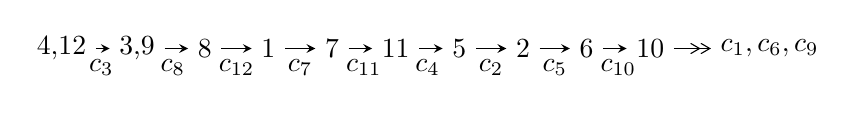
\begin{tikzpicture}[x=23pt, y=7pt]
	% node
	\node (A0) at (-1/8, 0) {4,12};
	\node (A1) at (17/16, 0) {3,9};
	\node (A2) at (17/8, 0) {8};
	\node (A3) at (25/8, 0) {1};
	\node (A4) at (33/8, 0) {7};
	\node (A5) at (41/8, 0) {11};
	\node (A6) at (49/8, 0) {5};
	\node (A7) at (57/8, 0) {2};
	\node (A8) at (65/8, 0) {6};
	\node (A9) at (73/8, 0) {10};
	\node (C1) at (1/2, -1) {$c_{3}$};
	\node (C2) at (13/8, -1) {$c_{8}$};
	\node (C3) at (21/8, -1) {$c_{12}$};
	\node (C4) at (29/8, -1) {$c_{7}$};
	\node (C5) at (37/8, -1) {$c_{11}$};
	\node (C6) at (45/8, -1) {$c_{4}$};
	\node (C7) at (53/8, -1) {$c_{2}$};
	\node (C8) at (61/8, -1) {$c_{5}$};
	\node (C9) at (69/8, -1) {$c_{10}$};
	\node (A10) at (11, 0) {$c_{1},c_{6},c_{9}$};

	% edge
	\draw[->,>=stealth]	
	(A0) edge (A1) (A1) edge (A2) (A2) edge (A3) (A3) edge (A4) (A4) edge (A5) (A5) edge (A6) (A6) edge (A7) (A7) edge (A8) (A8) edge (A9) ;
	\draw[->>,>={angle 60}]	
	(A9) edge (A10);
\end{tikzpicture} \\ 

\end{tabular} \\

\footnotetext{
The image of knot diagram is generated by the software ``\textbf{Draw programme}" developed by Andrew Bartholomew(\url{http://www.layer8.co.uk/maths/draw/index.htm\#Running-draw}), where we modified some parts for our purpose(\url{https://github.com/CATsTAILs/LinksPainter}).
}\phantom \\ \newline 
\centering \textbf{Ideals for irreducible components\footnotemark of $X_{\text{par}}$} 
 
\begin{align*}
I^u_{1}&=\langle 
1448 u^{11}-622 u^{10}+\cdots+1059 b-1564,\;a+1,\\
\phantom{I^u_{1}}&\phantom{= \langle  }u^{12}- u^{11}+2 u^9+4 u^8-4 u^7-3 u^6+9 u^5+u^4-4 u^3+5 u^2-2 u+1\rangle \\
I^u_{2}&=\langle 
u^4+u^3+2 u^2+b+u+2,\;a+1,\;u^5+u^4+2 u^3+2 u-1\rangle \\
I^u_{3}&=\langle 
-28 u^9-75 u^8-50 u^7+61 u^6-14 u^5-212 u^4-214 u^3-47 u^2+23 b-10 u+13,\\
\phantom{I^u_{3}}&\phantom{= \langle  }20 u^9+70 u^8+108 u^7+55 u^6+10 u^5+89 u^4+304 u^3+372 u^2+23 a+224 u+17,\\
\phantom{I^u_{3}}&\phantom{= \langle  }u^{10}+4 u^9+6 u^8+2 u^7- u^6+7 u^5+18 u^4+17 u^3+9 u^2+3 u+1\rangle \\
I^u_{4}&=\langle 
b-1,\;a+1,\;u^2+u+1\rangle \\
I^u_{5}&=\langle 
38 u^9-23 u^8+194 u^7-237 u^6+606 u^5+194 u^4+1010 u^3+389 u^2+563 b+442 u+545,\\
\phantom{I^u_{5}}&\phantom{= \langle  }412 u^9-842 u^8+1570 u^7-1651 u^6+4022 u^5-2371 u^4+4076 u^3-2894 u^2+1689 a+1592 u-3425,\\
\phantom{I^u_{5}}&\phantom{= \langle  }u^{10}-2 u^9+4 u^8-4 u^7+11 u^6-7 u^5+14 u^4-5 u^3+11 u^2-5 u+3\rangle \\
\\
\end{align*}
\raggedright * 5 irreducible components of $\dim_{\mathbb{C}}=0$, with total 39 representations.\\
\footnotetext{All coefficients of polynomials are rational numbers. But the coefficients are sometimes approximated in decimal forms when there is not enough margin.}
\newpage
\renewcommand{\arraystretch}{1}
\centering \section*{I. $I^u_{1}= \langle 1448 u^{11}-622 u^{10}+\cdots+1059 b-1564,\;a+1,\;u^{12}- u^{11}+\cdots-2 u+1 \rangle$}
\flushleft \textbf{(i) Arc colorings}\\
\begin{tabular}{m{7pt} m{180pt} m{7pt} m{180pt} }
\flushright $a_{4}=$&$\begin{pmatrix}1\\0\end{pmatrix}$ \\
\flushright $a_{12}=$&$\begin{pmatrix}0\\u\end{pmatrix}$ \\
\flushright $a_{3}=$&$\begin{pmatrix}1\\- u^2\end{pmatrix}$ \\
\flushright $a_{9}=$&$\begin{pmatrix}-1\\-1.36733 u^{11}+0.587347 u^{10}+\cdots-1.97734 u+1.47686\end{pmatrix}$ \\
\flushright $a_{8}=$&$\begin{pmatrix}-1.36733 u^{11}+0.587347 u^{10}+\cdots-1.97734 u+0.476865\\-1.36733 u^{11}+0.587347 u^{10}+\cdots-1.97734 u+1.47686\end{pmatrix}$ \\
\flushright $a_{1}=$&$\begin{pmatrix}-1.41171 u^{11}+0.928234 u^{10}+\cdots-3.16997 u+2.25685\\-2.19169 u^{11}+1.66383 u^{10}+\cdots-4.42776 u+3.62417\end{pmatrix}$ \\
\flushright $a_{7}=$&$\begin{pmatrix}0.0443815 u^{11}-0.340888 u^{10}+\cdots+0.192635 u-1.77998\\-1.20113 u^{11}+0.864023 u^{10}+\cdots-1.53258 u+1.96034\end{pmatrix}$ \\
\flushright $a_{11}=$&$\begin{pmatrix}u\\0.779981 u^{11}-0.735600 u^{10}+\cdots+2.25779 u-1.36733\end{pmatrix}$ \\
\flushright $a_{5}=$&$\begin{pmatrix}-0.0443815 u^{11}+0.340888 u^{10}+\cdots-0.192635 u+1.77998\\0.483475 u^{11}-0.649669 u^{10}+\cdots+0.566572 u-1.41171\end{pmatrix}$ \\
\flushright $a_{2}=$&$\begin{pmatrix}0.613787 u^{11}-1.01228 u^{10}+\cdots+0.813031 u-1.85080\\-1.47498 u^{11}+1.66950 u^{10}+\cdots-2.57224 u+3.70916\end{pmatrix}$ \\
\flushright $a_{6}=$&$\begin{pmatrix}-0.972616 u^{11}+2.61945 u^{10}+\cdots-1.79603 u+6.62512\\3.39754 u^{11}-4.62795 u^{10}+\cdots+6.51275 u-9.75260\end{pmatrix}$ \\
\flushright $a_{10}=$&$\begin{pmatrix}-0.613787 u^{11}+1.01228 u^{10}+\cdots-0.813031 u+1.85080\\1.37205 u^{11}-1.68744 u^{10}+\cdots+3.52975 u-3.64495\end{pmatrix}$\\&\end{tabular}
\flushleft \textbf{(ii) Obstruction class $= -1$}\\~\\
\flushleft \textbf{(iii) Cusp Shapes $= \frac{2459}{1059} u^{11}+\frac{3149}{1059} u^{10}-\frac{3035}{1059} u^9+\frac{1248}{353} u^8+\frac{20198}{1059} u^7+\frac{17837}{1059} u^6-\frac{17579}{1059} u^5+\frac{1070}{1059} u^4+\frac{14089}{353} u^3+\frac{14917}{1059} u^2+\frac{238}{353} u+\frac{13700}{1059}$}\\~\\
\newpage\renewcommand{\arraystretch}{1}
\flushleft \textbf{(iv) u-Polynomials at the component}\newline \\
\begin{tabular}{m{50pt}|m{274pt}}
Crossings & \hspace{64pt}u-Polynomials at each crossing \\
\hline $$\begin{aligned}c_{1}\end{aligned}$$&$\begin{aligned}
&u^{12}-12 u^{11}+\cdots+u+1
\end{aligned}$\\
\hline $$\begin{aligned}c_{2},c_{5},c_{6}\\c_{9}\end{aligned}$$&$\begin{aligned}
&u^{12}-6 u^{10}+\cdots- u+1
\end{aligned}$\\
\hline $$\begin{aligned}c_{3},c_{11}\end{aligned}$$&$\begin{aligned}
&u^{12}- u^{11}+2 u^9+4 u^8-4 u^7-3 u^6+9 u^5+u^4-4 u^3+5 u^2-2 u+1
\end{aligned}$\\
\hline $$\begin{aligned}c_{4},c_{10},c_{12}\end{aligned}$$&$\begin{aligned}
&u^{12}+u^{10}+12 u^9+21 u^8+30 u^7+38 u^6+39 u^5+33 u^4+4 u^3+4 u+4
\end{aligned}$\\
\hline $$\begin{aligned}c_{7}\end{aligned}$$&$\begin{aligned}
&u^{12}- u^{11}+\cdots-184 u+141
\end{aligned}$\\
\hline $$\begin{aligned}c_{8}\end{aligned}$$&$\begin{aligned}
&u^{12}-15 u^{11}+\cdots-576 u+96
\end{aligned}$\\
\hline
\end{tabular}\\~\\
\newpage\renewcommand{\arraystretch}{1}
\flushleft \textbf{(v) Riley Polynomials at the component}\newline \\
\begin{tabular}{m{50pt}|m{274pt}}
Crossings & \hspace{64pt}Riley Polynomials at each crossing \\
\hline $$\begin{aligned}c_{1}\end{aligned}$$&$\begin{aligned}
&y^{12}+36 y^{11}+\cdots+133 y+1
\end{aligned}$\\
\hline $$\begin{aligned}c_{2},c_{5},c_{6}\\c_{9}\end{aligned}$$&$\begin{aligned}
&y^{12}-12 y^{11}+\cdots+y+1
\end{aligned}$\\
\hline $$\begin{aligned}c_{3},c_{11}\end{aligned}$$&$\begin{aligned}
&y^{12}- y^{11}+\cdots+6 y+1
\end{aligned}$\\
\hline $$\begin{aligned}c_{4},c_{10},c_{12}\end{aligned}$$&$\begin{aligned}
&y^{12}+2 y^{11}+\cdots-16 y+16
\end{aligned}$\\
\hline $$\begin{aligned}c_{7}\end{aligned}$$&$\begin{aligned}
&y^{12}-23 y^{11}+\cdots+130832 y+19881
\end{aligned}$\\
\hline $$\begin{aligned}c_{8}\end{aligned}$$&$\begin{aligned}
&y^{12}-13 y^{11}+\cdots+10752 y+9216
\end{aligned}$\\
\hline
\end{tabular}\\~\\
\newpage\flushleft \textbf{(vi) Complex Volumes and Cusp Shapes}
$$\begin{array}{c|c|c}  
\text{Solutions to }I^u_{1}& \I (\text{vol} + \sqrt{-1}CS) & \text{Cusp shape}\\
 \hline 
\begin{aligned}
u &= -1.059120 + 0.307461 I \\
a &= -1.00000\phantom{ +0.000000I} \\
b &= \phantom{-}0.644594 - 0.475500 I\end{aligned}
 & -3.44334 + 1.44611 I & -3.96135 - 4.34110 I \\ \hline\begin{aligned}
u &= -1.059120 - 0.307461 I \\
a &= -1.00000\phantom{ +0.000000I} \\
b &= \phantom{-}0.644594 + 0.475500 I\end{aligned}
 & -3.44334 - 1.44611 I & -3.96135 + 4.34110 I \\ \hline\begin{aligned}
u &= \phantom{-}0.962226 + 0.662974 I \\
a &= -1.00000\phantom{ +0.000000I} \\
b &= \phantom{-}1.29438 + 1.01679 I\end{aligned}
 & -8.42695 - 4.69761 I & -5.39873 + 4.74294 I \\ \hline\begin{aligned}
u &= \phantom{-}0.962226 - 0.662974 I \\
a &= -1.00000\phantom{ +0.000000I} \\
b &= \phantom{-}1.29438 - 1.01679 I\end{aligned}
 & -8.42695 + 4.69761 I & -5.39873 - 4.74294 I \\ \hline\begin{aligned}
u &= \phantom{-}0.441542 + 0.466191 I \\
a &= -1.00000\phantom{ +0.000000I} \\
b &= \phantom{-}2.80322 - 1.33490 I\end{aligned}
 & \phantom{-}7.39753 - 0.41539 I & \phantom{-}6.7393 + 12.7489 I \\ \hline\begin{aligned}
u &= \phantom{-}0.441542 - 0.466191 I \\
a &= -1.00000\phantom{ +0.000000I} \\
b &= \phantom{-}2.80322 + 1.33490 I\end{aligned}
 & \phantom{-}7.39753 + 0.41539 I & \phantom{-}6.7393 - 12.7489 I \\ \hline\begin{aligned}
u &= -0.93584 + 1.09970 I \\
a &= -1.00000\phantom{ +0.000000I} \\
b &= \phantom{-}1.28519 - 0.74878 I\end{aligned}
 & -2.29460 + 6.83767 I & \phantom{-}0.069399 - 0.397217 I \\ \hline\begin{aligned}
u &= -0.93584 - 1.09970 I \\
a &= -1.00000\phantom{ +0.000000I} \\
b &= \phantom{-}1.28519 + 0.74878 I\end{aligned}
 & -2.29460 - 6.83767 I & \phantom{-}0.069399 + 0.397217 I \\ \hline\begin{aligned}
u &= \phantom{-}0.037712 + 0.516478 I \\
a &= -1.00000\phantom{ +0.000000I} \\
b &= \phantom{-}0.213856 + 0.762227 I\end{aligned}
 & \phantom{-}0.825162 + 0.816210 I & \phantom{-}7.49070 - 5.15552 I \\ \hline\begin{aligned}
u &= \phantom{-}0.037712 - 0.516478 I \\
a &= -1.00000\phantom{ +0.000000I} \\
b &= \phantom{-}0.213856 - 0.762227 I\end{aligned}
 & \phantom{-}0.825162 - 0.816210 I & \phantom{-}7.49070 + 5.15552 I\\
 \hline 
 \end{array}$$\newpage$$\begin{array}{c|c|c}  
\text{Solutions to }I^u_{1}& \I (\text{vol} + \sqrt{-1}CS) & \text{Cusp shape}\\
 \hline 
\begin{aligned}
u &= \phantom{-}1.05347 + 1.22560 I \\
a &= -1.00000\phantom{ +0.000000I} \\
b &= \phantom{-}1.25877 + 1.59603 I\end{aligned}
 & \phantom{-}10.0545 - 12.2992 I & \phantom{-}3.06065 + 5.11148 I \\ \hline\begin{aligned}
u &= \phantom{-}1.05347 - 1.22560 I \\
a &= -1.00000\phantom{ +0.000000I} \\
b &= \phantom{-}1.25877 - 1.59603 I\end{aligned}
 & \phantom{-}10.0545 + 12.2992 I & \phantom{-}3.06065 - 5.11148 I\\
 \hline 
 \end{array}$$\newpage\newpage\renewcommand{\arraystretch}{1}
\centering \section*{II. $I^u_{2}= \langle u^4+u^3+2 u^2+b+u+2,\;a+1,\;u^5+u^4+2 u^3+2 u-1 \rangle$}
\flushleft \textbf{(i) Arc colorings}\\
\begin{tabular}{m{7pt} m{180pt} m{7pt} m{180pt} }
\flushright $a_{4}=$&$\begin{pmatrix}1\\0\end{pmatrix}$ \\
\flushright $a_{12}=$&$\begin{pmatrix}0\\u\end{pmatrix}$ \\
\flushright $a_{3}=$&$\begin{pmatrix}1\\- u^2\end{pmatrix}$ \\
\flushright $a_{9}=$&$\begin{pmatrix}-1\\- u^4- u^3-2 u^2- u-2\end{pmatrix}$ \\
\flushright $a_{8}=$&$\begin{pmatrix}- u^4- u^3-2 u^2- u-3\\- u^4- u^3-2 u^2- u-2\end{pmatrix}$ \\
\flushright $a_{1}=$&$\begin{pmatrix}u^4+2 u^3+4 u^2+3 u+4\\u^4+2 u^3+3 u^2+3 u+3\end{pmatrix}$ \\
\flushright $a_{7}=$&$\begin{pmatrix}u^3+u^2+u-1\\- u^4- u^3-2 u^2-3\end{pmatrix}$ \\
\flushright $a_{11}=$&$\begin{pmatrix}u\\u^2+u+1\end{pmatrix}$ \\
\flushright $a_{5}=$&$\begin{pmatrix}- u^3- u^2- u+1\\- u^4-2 u^3-3 u^2-2 u-1\end{pmatrix}$ \\
\flushright $a_{2}=$&$\begin{pmatrix}- u^4- u^3- u^2+u\\u^4+2 u^3+3 u^2+3 u+4\end{pmatrix}$ \\
\flushright $a_{6}=$&$\begin{pmatrix}0\\-5 u^4-7 u^3-13 u^2-5 u-12\end{pmatrix}$ \\
\flushright $a_{10}=$&$\begin{pmatrix}u^4+u^3+u^2- u\\2 u^4+3 u^3+5 u^2+u+4\end{pmatrix}$\\&\end{tabular}
\flushleft \textbf{(ii) Obstruction class $= 1$}\\~\\
\flushleft \textbf{(iii) Cusp Shapes $= u^4+10 u^2+u+10$}\\~\\
\newpage\renewcommand{\arraystretch}{1}
\flushleft \textbf{(iv) u-Polynomials at the component}\newline \\
\begin{tabular}{m{50pt}|m{274pt}}
Crossings & \hspace{64pt}u-Polynomials at each crossing \\
\hline $$\begin{aligned}c_{1}\end{aligned}$$&$\begin{aligned}
&u^5+4 u^4-10 u^3+8 u^2-3 u+1
\end{aligned}$\\
\hline $$\begin{aligned}c_{2},c_{6}\end{aligned}$$&$\begin{aligned}
&u^5+2 u^4+2 u^2- u+1
\end{aligned}$\\
\hline $$\begin{aligned}c_{3},c_{11}\end{aligned}$$&$\begin{aligned}
&u^5+u^4+2 u^3+2 u-1
\end{aligned}$\\
\hline $$\begin{aligned}c_{4},c_{12}\end{aligned}$$&$\begin{aligned}
&u^5- u^4+2 u^3-3 u^2-4
\end{aligned}$\\
\hline $$\begin{aligned}c_{5},c_{9}\end{aligned}$$&$\begin{aligned}
&u^5-2 u^4-2 u^2- u-1
\end{aligned}$\\
\hline $$\begin{aligned}c_{7}\end{aligned}$$&$\begin{aligned}
&u^5-2 u^4-4 u^3-3 u^2-3 u-5
\end{aligned}$\\
\hline $$\begin{aligned}c_{8}\end{aligned}$$&$\begin{aligned}
&u^5- u^4-5 u^3-2 u^2+4 u-1
\end{aligned}$\\
\hline $$\begin{aligned}c_{10}\end{aligned}$$&$\begin{aligned}
&u^5+u^4+2 u^3+3 u^2+4
\end{aligned}$\\
\hline
\end{tabular}\\~\\
\newpage\renewcommand{\arraystretch}{1}
\flushleft \textbf{(v) Riley Polynomials at the component}\newline \\
\begin{tabular}{m{50pt}|m{274pt}}
Crossings & \hspace{64pt}Riley Polynomials at each crossing \\
\hline $$\begin{aligned}c_{1}\end{aligned}$$&$\begin{aligned}
&y^5-36 y^4+30 y^3-12 y^2-7 y-1
\end{aligned}$\\
\hline $$\begin{aligned}c_{2},c_{5},c_{6}\\c_{9}\end{aligned}$$&$\begin{aligned}
&y^5-4 y^4-10 y^3-8 y^2-3 y-1
\end{aligned}$\\
\hline $$\begin{aligned}c_{3},c_{11}\end{aligned}$$&$\begin{aligned}
&y^5+3 y^4+8 y^3+10 y^2+4 y-1
\end{aligned}$\\
\hline $$\begin{aligned}c_{4},c_{10},c_{12}\end{aligned}$$&$\begin{aligned}
&y^5+3 y^4-2 y^3-17 y^2-24 y-16
\end{aligned}$\\
\hline $$\begin{aligned}c_{7}\end{aligned}$$&$\begin{aligned}
&y^5-12 y^4-2 y^3-5 y^2-21 y-25
\end{aligned}$\\
\hline $$\begin{aligned}c_{8}\end{aligned}$$&$\begin{aligned}
&y^5-11 y^4+29 y^3-46 y^2+12 y-1
\end{aligned}$\\
\hline
\end{tabular}\\~\\
\newpage\flushleft \textbf{(vi) Complex Volumes and Cusp Shapes}
$$\begin{array}{c|c|c}  
\text{Solutions to }I^u_{2}& \I (\text{vol} + \sqrt{-1}CS) & \text{Cusp shape}\\
 \hline 
\begin{aligned}
u &= \phantom{-}0.205345 + 1.022070 I \\
a &= -1.00000\phantom{ +0.000000I} \\
b &= -0.394292 - 0.081621 I\end{aligned}
 & -4.76566 - 1.63339 I & \phantom{-}1.00951 + 4.37803 I \\ \hline\begin{aligned}
u &= \phantom{-}0.205345 - 1.022070 I \\
a &= -1.00000\phantom{ +0.000000I} \\
b &= -0.394292 + 0.081621 I\end{aligned}
 & -4.76566 + 1.63339 I & \phantom{-}1.00951 - 4.37803 I \\ \hline\begin{aligned}
u &= -0.91068 + 1.18795 I \\
a &= -1.00000\phantom{ +0.000000I} \\
b &= \phantom{-}1.31714 - 0.65774 I\end{aligned}
 & -2.30891 + 7.29116 I & -1.0723 - 17.9309 I \\ \hline\begin{aligned}
u &= -0.91068 - 1.18795 I \\
a &= -1.00000\phantom{ +0.000000I} \\
b &= \phantom{-}1.31714 + 0.65774 I\end{aligned}
 & -2.30891 - 7.29116 I & -1.0723 + 17.9309 I \\ \hline\begin{aligned}
u &= \phantom{-}0.410675\phantom{ +0.000000I} \\
a &= -1.00000\phantom{ +0.000000I} \\
b &= -2.84569\phantom{ +0.000000I}\end{aligned}
 & \phantom{-}7.56942\phantom{ +0.000000I} & \phantom{-}12.1260\phantom{ +0.000000I}\\
 \hline 
 \end{array}$$\newpage\newpage\renewcommand{\arraystretch}{1}
\centering \section*{III. $I^u_{3}= \langle -28 u^9-75 u^8+\cdots+23 b+13,\;20 u^9+70 u^8+\cdots+23 a+17,\;u^{10}+4 u^9+\cdots+3 u+1 \rangle$}
\flushleft \textbf{(i) Arc colorings}\\
\begin{tabular}{m{7pt} m{180pt} m{7pt} m{180pt} }
\flushright $a_{4}=$&$\begin{pmatrix}1\\0\end{pmatrix}$ \\
\flushright $a_{12}=$&$\begin{pmatrix}0\\u\end{pmatrix}$ \\
\flushright $a_{3}=$&$\begin{pmatrix}1\\- u^2\end{pmatrix}$ \\
\flushright $a_{9}=$&$\begin{pmatrix}-0.869565 u^{9}-3.04348 u^{8}+\cdots-9.73913 u-0.739130\\1.21739 u^{9}+3.26087 u^{8}+\cdots+0.434783 u-0.565217\end{pmatrix}$ \\
\flushright $a_{8}=$&$\begin{pmatrix}0.347826 u^{9}+0.217391 u^{8}+\cdots-9.30435 u-1.30435\\1.21739 u^{9}+3.26087 u^{8}+\cdots+0.434783 u-0.565217\end{pmatrix}$ \\
\flushright $a_{1}=$&$\begin{pmatrix}-2.91304 u^{9}-11.6957 u^{8}+\cdots-20.8261 u-2.82609\\-0.130435 u^{9}+0.0434783 u^{8}+\cdots-1.26087 u-0.260870\end{pmatrix}$ \\
\flushright $a_{7}=$&$\begin{pmatrix}-0.956522 u^{9}-4.34783 u^{8}+\cdots-12.9130 u-1.91304\\1.04348 u^{9}+3.65217 u^{8}+\cdots+1.08696 u+0.0869565\end{pmatrix}$ \\
\flushright $a_{11}=$&$\begin{pmatrix}-1.13043 u^{9}-5.95652 u^{8}+\cdots-11.2609 u-0.260870\\-1.65217 u^{9}-5.78261 u^{8}+\cdots-6.30435 u-2.30435\end{pmatrix}$ \\
\flushright $a_{5}=$&$\begin{pmatrix}-2.82609 u^{9}-9.39130 u^{8}+\cdots+3.34783 u+2.34783\\-0.565217 u^{9}-1.47826 u^{8}+\cdots-1.13043 u+0.869565\end{pmatrix}$ \\
\flushright $a_{2}=$&$\begin{pmatrix}-3.30435 u^{9}-13.5652 u^{8}+\cdots-22.6087 u-2.60870\\-0.782609 u^{9}-1.73913 u^{8}+\cdots-2.56522 u-0.565217\end{pmatrix}$ \\
\flushright $a_{6}=$&$\begin{pmatrix}-2.65217 u^{9}-9.78261 u^{8}+\cdots-16.3043 u-6.30435\\-0.304348 u^{9}+0.434783 u^{8}+\cdots+1.39130 u+1.39130\end{pmatrix}$ \\
\flushright $a_{10}=$&$\begin{pmatrix}-1.34783 u^{9}-3.21739 u^{8}+\cdots+3.30435 u+3.30435\\1.95652 u^{9}+6.34783 u^{8}+\cdots+3.91304 u+1.91304\end{pmatrix}$\\&\end{tabular}
\flushleft \textbf{(ii) Obstruction class $= 1$}\\~\\
\flushleft \textbf{(iii) Cusp Shapes $= -\frac{122}{23} u^9-\frac{289}{23} u^8-\frac{139}{23} u^7+\frac{297}{23} u^6-\frac{107}{23} u^5-\frac{835}{23} u^4-\frac{755}{23} u^3-\frac{75}{23} u^2+\frac{101}{23} u+\frac{124}{23}$}\\~\\
\newpage\renewcommand{\arraystretch}{1}
\flushleft \textbf{(iv) u-Polynomials at the component}\newline \\
\begin{tabular}{m{50pt}|m{274pt}}
Crossings & \hspace{64pt}u-Polynomials at each crossing \\
\hline $$\begin{aligned}c_{1}\end{aligned}$$&$\begin{aligned}
&u^{10}-9 u^9+31 u^8-56 u^7+73 u^6-86 u^5+65 u^4-12 u^3-9 u^2+2 u+1
\end{aligned}$\\
\hline $$\begin{aligned}c_{2},c_{6}\end{aligned}$$&$\begin{aligned}
&u^{10}+u^9+5 u^8+4 u^7+7 u^6+2 u^5+3 u^4-4 u^3+u^2-2 u+1
\end{aligned}$\\
\hline $$\begin{aligned}c_{3},c_{11}\end{aligned}$$&$\begin{aligned}
&u^{10}+4 u^9+6 u^8+2 u^7- u^6+7 u^5+18 u^4+17 u^3+9 u^2+3 u+1
\end{aligned}$\\
\hline $$\begin{aligned}c_{4},c_{12}\end{aligned}$$&$\begin{aligned}
&u^{10}+3 u^9+6 u^8+8 u^7+7 u^6+2 u^5+6 u^4+5 u^3+15 u^2+7 u+7
\end{aligned}$\\
\hline $$\begin{aligned}c_{5},c_{9}\end{aligned}$$&$\begin{aligned}
&u^{10}- u^9+5 u^8-4 u^7+7 u^6-2 u^5+3 u^4+4 u^3+u^2+2 u+1
\end{aligned}$\\
\hline $$\begin{aligned}c_{7}\end{aligned}$$&$\begin{aligned}
&u^{10}-3 u^9+\cdots-66 u+17
\end{aligned}$\\
\hline $$\begin{aligned}c_{8}\end{aligned}$$&$\begin{aligned}
&(u^5-3 u^4+4 u^3- u^2- u+1)^2
\end{aligned}$\\
\hline $$\begin{aligned}c_{10}\end{aligned}$$&$\begin{aligned}
&u^{10}-3 u^9+6 u^8-8 u^7+7 u^6-2 u^5+6 u^4-5 u^3+15 u^2-7 u+7
\end{aligned}$\\
\hline
\end{tabular}\\~\\
\newpage\renewcommand{\arraystretch}{1}
\flushleft \textbf{(v) Riley Polynomials at the component}\newline \\
\begin{tabular}{m{50pt}|m{274pt}}
Crossings & \hspace{64pt}Riley Polynomials at each crossing \\
\hline $$\begin{aligned}c_{1}\end{aligned}$$&$\begin{aligned}
&y^{10}-19 y^9+\cdots-22 y+1
\end{aligned}$\\
\hline $$\begin{aligned}c_{2},c_{5},c_{6}\\c_{9}\end{aligned}$$&$\begin{aligned}
&y^{10}+9 y^9+31 y^8+56 y^7+73 y^6+86 y^5+65 y^4+12 y^3-9 y^2-2 y+1
\end{aligned}$\\
\hline $$\begin{aligned}c_{3},c_{11}\end{aligned}$$&$\begin{aligned}
&y^{10}-4 y^9+18 y^8-36 y^7+71 y^6-67 y^5+68 y^4-9 y^3+15 y^2+9 y+1
\end{aligned}$\\
\hline $$\begin{aligned}c_{4},c_{10},c_{12}\end{aligned}$$&$\begin{aligned}
&y^{10}+3 y^9+\cdots+161 y+49
\end{aligned}$\\
\hline $$\begin{aligned}c_{7}\end{aligned}$$&$\begin{aligned}
&y^{10}+21 y^9+\cdots+302 y+289
\end{aligned}$\\
\hline $$\begin{aligned}c_{8}\end{aligned}$$&$\begin{aligned}
&(y^5- y^4+8 y^3-3 y^2+3 y-1)^2
\end{aligned}$\\
\hline
\end{tabular}\\~\\
\newpage\flushleft \textbf{(vi) Complex Volumes and Cusp Shapes}
$$\begin{array}{c|c|c}  
\text{Solutions to }I^u_{3}& \I (\text{vol} + \sqrt{-1}CS) & \text{Cusp shape}\\
 \hline 
\begin{aligned}
u &= -0.637527 + 0.563270 I \\
a &= \phantom{-}1.53949 + 0.13288 I \\
b &= -1.23271 + 1.09381 I\end{aligned}
 & -7.51750 + 4.40083 I & \phantom{-}4.55516 - 1.78781 I \\ \hline\begin{aligned}
u &= -0.637527 - 0.563270 I \\
a &= \phantom{-}1.53949 - 0.13288 I \\
b &= -1.23271 - 1.09381 I\end{aligned}
 & -7.51750 - 4.40083 I & \phantom{-}4.55516 + 1.78781 I \\ \hline\begin{aligned}
u &= -1.108870 + 0.598693 I \\
a &= -0.548579 - 0.836099 I \\
b &= \phantom{-}0.588022\phantom{ +0.000000I}\end{aligned}
 & -4.04602\phantom{ +0.000000I} & -7.96494 + 0. I\phantom{ +0.000000I} \\ \hline\begin{aligned}
u &= -1.108870 - 0.598693 I \\
a &= -0.548579 + 0.836099 I \\
b &= \phantom{-}0.588022\phantom{ +0.000000I}\end{aligned}
 & -4.04602\phantom{ +0.000000I} & -7.96494 + 0. I\phantom{ +0.000000I} \\ \hline\begin{aligned}
u &= \phantom{-}1.056310 + 0.782435 I \\
a &= \phantom{-}0.644763 + 0.055651 I \\
b &= -1.23271 - 1.09381 I\end{aligned}
 & -7.51750 - 4.40083 I & \phantom{-}4.55516 + 1.78781 I \\ \hline\begin{aligned}
u &= \phantom{-}1.056310 - 0.782435 I \\
a &= \phantom{-}0.644763 - 0.055651 I \\
b &= -1.23271 + 1.09381 I\end{aligned}
 & -7.51750 + 4.40083 I & \phantom{-}4.55516 - 1.78781 I \\ \hline\begin{aligned}
u &= -0.008215 + 0.434693 I \\
a &= \phantom{-}2.20767 - 3.03625 I \\
b &= -0.561306 - 0.557752 I\end{aligned}
 & -1.97403 - 1.53058 I & \phantom{-}4.42731 + 4.45807 I \\ \hline\begin{aligned}
u &= -0.008215 - 0.434693 I \\
a &= \phantom{-}2.20767 + 3.03625 I \\
b &= -0.561306 + 0.557752 I\end{aligned}
 & -1.97403 + 1.53058 I & \phantom{-}4.42731 - 4.45807 I \\ \hline\begin{aligned}
u &= -1.30170 + 0.98460 I \\
a &= \phantom{-}0.156654 - 0.215449 I \\
b &= -0.561306 + 0.557752 I\end{aligned}
 & -1.97403 + 1.53058 I & \phantom{-}4.42731 - 4.45807 I \\ \hline\begin{aligned}
u &= -1.30170 - 0.98460 I \\
a &= \phantom{-}0.156654 + 0.215449 I \\
b &= -0.561306 - 0.557752 I\end{aligned}
 & -1.97403 - 1.53058 I & \phantom{-}4.42731 + 4.45807 I\\
 \hline 
 \end{array}$$\newpage\newpage\renewcommand{\arraystretch}{1}
\centering \section*{IV. $I^u_{4}= \langle b-1,\;a+1,\;u^2+u+1 \rangle$}
\flushleft \textbf{(i) Arc colorings}\\
\begin{tabular}{m{7pt} m{180pt} m{7pt} m{180pt} }
\flushright $a_{4}=$&$\begin{pmatrix}1\\0\end{pmatrix}$ \\
\flushright $a_{12}=$&$\begin{pmatrix}0\\u\end{pmatrix}$ \\
\flushright $a_{3}=$&$\begin{pmatrix}1\\u+1\end{pmatrix}$ \\
\flushright $a_{9}=$&$\begin{pmatrix}-1\\1\end{pmatrix}$ \\
\flushright $a_{8}=$&$\begin{pmatrix}0\\1\end{pmatrix}$ \\
\flushright $a_{1}=$&$\begin{pmatrix}0\\u\end{pmatrix}$ \\
\flushright $a_{7}=$&$\begin{pmatrix}-1\\- u\end{pmatrix}$ \\
\flushright $a_{11}=$&$\begin{pmatrix}u\\0\end{pmatrix}$ \\
\flushright $a_{5}=$&$\begin{pmatrix}1\\0\end{pmatrix}$ \\
\flushright $a_{2}=$&$\begin{pmatrix}- u\\u+1\end{pmatrix}$ \\
\flushright $a_{6}=$&$\begin{pmatrix}0\\- u\end{pmatrix}$ \\
\flushright $a_{10}=$&$\begin{pmatrix}u\\0\end{pmatrix}$\\&\end{tabular}
\flushleft \textbf{(ii) Obstruction class $= 1$}\\~\\
\flushleft \textbf{(iii) Cusp Shapes $= -8 u+2$}\\~\\
\newpage\renewcommand{\arraystretch}{1}
\flushleft \textbf{(iv) u-Polynomials at the component}\newline \\
\begin{tabular}{m{50pt}|m{274pt}}
Crossings & \hspace{64pt}u-Polynomials at each crossing \\
\hline $$\begin{aligned}c_{1},c_{5},c_{9}\end{aligned}$$&$\begin{aligned}
&u^2- u+1
\end{aligned}$\\
\hline $$\begin{aligned}c_{2},c_{3},c_{6}\\c_{11}\end{aligned}$$&$\begin{aligned}
&u^2+u+1
\end{aligned}$\\
\hline $$\begin{aligned}c_{4},c_{10},c_{12}\end{aligned}$$&$\begin{aligned}
&u^2
\end{aligned}$\\
\hline $$\begin{aligned}c_{7},c_{8}\end{aligned}$$&$\begin{aligned}
&(u+1)^2
\end{aligned}$\\
\hline
\end{tabular}\\~\\
\newpage\renewcommand{\arraystretch}{1}
\flushleft \textbf{(v) Riley Polynomials at the component}\newline \\
\begin{tabular}{m{50pt}|m{274pt}}
Crossings & \hspace{64pt}Riley Polynomials at each crossing \\
\hline $$\begin{aligned}c_{1},c_{2},c_{3}\\c_{5},c_{6},c_{9}\\c_{11}\end{aligned}$$&$\begin{aligned}
&y^2+y+1
\end{aligned}$\\
\hline $$\begin{aligned}c_{4},c_{10},c_{12}\end{aligned}$$&$\begin{aligned}
&y^2
\end{aligned}$\\
\hline $$\begin{aligned}c_{7},c_{8}\end{aligned}$$&$\begin{aligned}
&(y-1)^2
\end{aligned}$\\
\hline
\end{tabular}\\~\\
\newpage\flushleft \textbf{(vi) Complex Volumes and Cusp Shapes}
$$\begin{array}{c|c|c}  
\text{Solutions to }I^u_{4}& \I (\text{vol} + \sqrt{-1}CS) & \text{Cusp shape}\\
 \hline 
\begin{aligned}
u &= -0.500000 + 0.866025 I \\
a &= -1.00000\phantom{ +0.000000I} \\
b &= \phantom{-}1.00000\phantom{ +0.000000I}\end{aligned}
 & \phantom{-0.000000 -}4.05977 I & \phantom{-}6.00000 - 6.92820 I \\ \hline\begin{aligned}
u &= -0.500000 - 0.866025 I \\
a &= -1.00000\phantom{ +0.000000I} \\
b &= \phantom{-}1.00000\phantom{ +0.000000I}\end{aligned}
 & \phantom{-0.000000 } -4.05977 I & \phantom{-}6.00000 + 6.92820 I\\
 \hline 
 \end{array}$$\newpage\newpage\renewcommand{\arraystretch}{1}
\centering \section*{V. $I^u_{5}= \langle 38 u^9-23 u^8+\cdots+563 b+545,\;412 u^9-842 u^8+\cdots+1689 a-3425,\;u^{10}-2 u^9+\cdots-5 u+3 \rangle$}
\flushleft \textbf{(i) Arc colorings}\\
\begin{tabular}{m{7pt} m{180pt} m{7pt} m{180pt} }
\flushright $a_{4}=$&$\begin{pmatrix}1\\0\end{pmatrix}$ \\
\flushright $a_{12}=$&$\begin{pmatrix}0\\u\end{pmatrix}$ \\
\flushright $a_{3}=$&$\begin{pmatrix}1\\- u^2\end{pmatrix}$ \\
\flushright $a_{9}=$&$\begin{pmatrix}-0.243931 u^{9}+0.498520 u^{8}+\cdots-0.942570 u+2.02783\\-0.0674956 u^{9}+0.0408526 u^{8}+\cdots-0.785080 u-0.968028\end{pmatrix}$ \\
\flushright $a_{8}=$&$\begin{pmatrix}-0.311427 u^{9}+0.539372 u^{8}+\cdots-1.72765 u+1.05980\\-0.0674956 u^{9}+0.0408526 u^{8}+\cdots-0.785080 u-0.968028\end{pmatrix}$ \\
\flushright $a_{1}=$&$\begin{pmatrix}-0.461220 u^{9}+1.11249 u^{8}+\cdots-3.36471 u+2.88514\\-0.346359 u^{9}+0.499112 u^{8}+\cdots-0.765542 u+0.216696\end{pmatrix}$ \\
\flushright $a_{7}=$&$\begin{pmatrix}-0.0485494 u^{9}+0.0118413 u^{8}+\cdots-1.45944 u+1.77738\\0.277087 u^{9}-0.799290 u^{8}+\cdots+0.0124334 u-0.973357\end{pmatrix}$ \\
\flushright $a_{11}=$&$\begin{pmatrix}0.169331 u^{9}+0.178212 u^{8}+\cdots+1.28538 u+1.84962\\-0.284192 u^{9}+0.435169 u^{8}+\cdots-1.88455 u+0.818828\end{pmatrix}$ \\
\flushright $a_{5}=$&$\begin{pmatrix}-0.366489 u^{9}+0.967436 u^{8}+\cdots-1.73653 u+0.612197\\-0.165187 u^{9}+0.284192 u^{8}+\cdots-1.02664 u+0.657194\end{pmatrix}$ \\
\flushright $a_{2}=$&$\begin{pmatrix}-0.985198 u^{9}+1.50858 u^{8}+\cdots-4.93310 u+3.23860\\-0.884547 u^{9}+0.166963 u^{8}+\cdots+0.921847 u-1.73890\end{pmatrix}$ \\
\flushright $a_{6}=$&$\begin{pmatrix}-4.03848 u^{9}+6.27768 u^{8}+\cdots-10.9739 u+2.57963\\-1.03197 u^{9}-0.138544 u^{8}+\cdots+0.575488 u-4.19538\end{pmatrix}$ \\
\flushright $a_{10}=$&$\begin{pmatrix}-1.07697 u^{9}+2.55536 u^{8}+\cdots-1.94790 u+3.15927\\-1.22025 u^{9}+1.71226 u^{8}+\cdots-4.03552 u+0.209591\end{pmatrix}$\\&\end{tabular}
\flushleft \textbf{(ii) Obstruction class $= -1$}\\~\\
\flushleft \textbf{(iii) Cusp Shapes $= \frac{630}{563} u^9-\frac{1211}{563} u^8+\frac{2357}{563} u^7-\frac{1855}{563} u^6+\frac{5691}{563} u^5-\frac{2147}{563} u^4+\frac{6107}{563} u^3+\frac{997}{563} u^2+\frac{3861}{563} u+\frac{2724}{563}$}\\~\\
\newpage\renewcommand{\arraystretch}{1}
\flushleft \textbf{(iv) u-Polynomials at the component}\newline \\
\begin{tabular}{m{50pt}|m{274pt}}
Crossings & \hspace{64pt}u-Polynomials at each crossing \\
\hline $$\begin{aligned}c_{1}\end{aligned}$$&$\begin{aligned}
&u^{10}-19 u^9+\cdots+2834 u+441
\end{aligned}$\\
\hline $$\begin{aligned}c_{2},c_{5},c_{6}\\c_{9}\end{aligned}$$&$\begin{aligned}
&u^{10}-3 u^9+\cdots+8 u+21
\end{aligned}$\\
\hline $$\begin{aligned}c_{3},c_{11}\end{aligned}$$&$\begin{aligned}
&u^{10}-2 u^9+4 u^8-4 u^7+11 u^6-7 u^5+14 u^4-5 u^3+11 u^2-5 u+3
\end{aligned}$\\
\hline $$\begin{aligned}c_{4},c_{10},c_{12}\end{aligned}$$&$\begin{aligned}
&u^{10}+u^9+\cdots+55 u+43
\end{aligned}$\\
\hline $$\begin{aligned}c_{7}\end{aligned}$$&$\begin{aligned}
&u^{10}+5 u^9+\cdots+248 u+59
\end{aligned}$\\
\hline $$\begin{aligned}c_{8}\end{aligned}$$&$\begin{aligned}
&(u^5- u^4+u^2+u-1)^2
\end{aligned}$\\
\hline
\end{tabular}\\~\\
\newpage\renewcommand{\arraystretch}{1}
\flushleft \textbf{(v) Riley Polynomials at the component}\newline \\
\begin{tabular}{m{50pt}|m{274pt}}
Crossings & \hspace{64pt}Riley Polynomials at each crossing \\
\hline $$\begin{aligned}c_{1}\end{aligned}$$&$\begin{aligned}
&y^{10}+173 y^9+\cdots+10034450 y+194481
\end{aligned}$\\
\hline $$\begin{aligned}c_{2},c_{5},c_{6}\\c_{9}\end{aligned}$$&$\begin{aligned}
&y^{10}-19 y^9+\cdots+2834 y+441
\end{aligned}$\\
\hline $$\begin{aligned}c_{3},c_{11}\end{aligned}$$&$\begin{aligned}
&y^{10}+4 y^9+\cdots+41 y+9
\end{aligned}$\\
\hline $$\begin{aligned}c_{4},c_{10},c_{12}\end{aligned}$$&$\begin{aligned}
&y^{10}+7 y^9+\cdots-875 y+1849
\end{aligned}$\\
\hline $$\begin{aligned}c_{7}\end{aligned}$$&$\begin{aligned}
&y^{10}-15 y^9+\cdots+9178 y+3481
\end{aligned}$\\
\hline $$\begin{aligned}c_{8}\end{aligned}$$&$\begin{aligned}
&(y^5- y^4+4 y^3-3 y^2+3 y-1)^2
\end{aligned}$\\
\hline
\end{tabular}\\~\\
\newpage\flushleft \textbf{(vi) Complex Volumes and Cusp Shapes}
$$\begin{array}{c|c|c}  
\text{Solutions to }I^u_{5}& \I (\text{vol} + \sqrt{-1}CS) & \text{Cusp shape}\\
 \hline 
\begin{aligned}
u &= -0.597158 + 0.899620 I \\
a &= \phantom{-}0.542169 + 0.003339 I \\
b &= -0.758138 + 0.584034 I\end{aligned}
 & \phantom{-}0.17487 + 2.21397 I & \phantom{-}5.11913 - 4.04855 I \\ \hline\begin{aligned}
u &= -0.597158 - 0.899620 I \\
a &= \phantom{-}0.542169 - 0.003339 I \\
b &= -0.758138 - 0.584034 I\end{aligned}
 & \phantom{-}0.17487 - 2.21397 I & \phantom{-}5.11913 + 4.04855 I \\ \hline\begin{aligned}
u &= \phantom{-}0.453573 + 1.045560 I \\
a &= \phantom{-}0.50995 + 1.56353 I \\
b &= \phantom{-}0.935538 + 0.903908 I\end{aligned}
 & \phantom{-}9.31336 - 3.33174 I & \phantom{-}4.71334 + 2.53508 I \\ \hline\begin{aligned}
u &= \phantom{-}0.453573 - 1.045560 I \\
a &= \phantom{-}0.50995 - 1.56353 I \\
b &= \phantom{-}0.935538 - 0.903908 I\end{aligned}
 & \phantom{-}9.31336 + 3.33174 I & \phantom{-}4.71334 - 2.53508 I \\ \hline\begin{aligned}
u &= -0.586646 + 1.140630 I \\
a &= \phantom{-}0.581627 - 0.813455 I \\
b &= \phantom{-}0.645200\phantom{ +0.000000I}\end{aligned}
 & -2.52712\phantom{ +0.000000I} & \phantom{-}4.33506 + 0. I\phantom{ +0.000000I} \\ \hline\begin{aligned}
u &= -0.586646 - 1.140630 I \\
a &= \phantom{-}0.581627 + 0.813455 I \\
b &= \phantom{-}0.645200\phantom{ +0.000000I}\end{aligned}
 & -2.52712\phantom{ +0.000000I} & \phantom{-}4.33506 + 0. I\phantom{ +0.000000I} \\ \hline\begin{aligned}
u &= \phantom{-}0.326764 + 0.485752 I \\
a &= \phantom{-}1.84438 + 0.01136 I \\
b &= -0.758138 - 0.584034 I\end{aligned}
 & \phantom{-}0.17487 - 2.21397 I & \phantom{-}5.11913 + 4.04855 I \\ \hline\begin{aligned}
u &= \phantom{-}0.326764 - 0.485752 I \\
a &= \phantom{-}1.84438 - 0.01136 I \\
b &= -0.758138 + 0.584034 I\end{aligned}
 & \phantom{-}0.17487 + 2.21397 I & \phantom{-}5.11913 - 4.04855 I \\ \hline\begin{aligned}
u &= \phantom{-}1.40347 + 1.24236 I \\
a &= \phantom{-}0.188544 + 0.578083 I \\
b &= \phantom{-}0.935538 - 0.903908 I\end{aligned}
 & \phantom{-}9.31336 + 3.33174 I & \phantom{-}4.71334 - 2.53508 I \\ \hline\begin{aligned}
u &= \phantom{-}1.40347 - 1.24236 I \\
a &= \phantom{-}0.188544 - 0.578083 I \\
b &= \phantom{-}0.935538 + 0.903908 I\end{aligned}
 & \phantom{-}9.31336 - 3.33174 I & \phantom{-}4.71334 + 2.53508 I\\
 \hline 
 \end{array}$$\newpage
\newpage\renewcommand{\arraystretch}{1}
\centering \section*{ VI. u-Polynomials}
\begin{tabular}{m{50pt}|m{274pt}}
Crossings & \hspace{64pt}u-Polynomials at each crossing \\
\hline $$\begin{aligned}c_{1}\end{aligned}$$&$\begin{aligned}
&(u^2- u+1)(u^5+4 u^4-10 u^3+8 u^2-3 u+1)\\
&\cdot(u^{10}-19 u^9+\cdots+2834 u+441)\\
&\cdot(u^{10}-9 u^9+31 u^8-56 u^7+73 u^6-86 u^5+65 u^4-12 u^3-9 u^2+2 u+1)\\
&\cdot(u^{12}-12 u^{11}+\cdots+u+1)
\end{aligned}$\\
\hline $$\begin{aligned}c_{2},c_{6}\end{aligned}$$&$\begin{aligned}
&(u^2+u+1)(u^5+2 u^4+2 u^2- u+1)(u^{10}-3 u^9+\cdots+8 u+21)\\
&\cdot(u^{10}+u^9+5 u^8+4 u^7+7 u^6+2 u^5+3 u^4-4 u^3+u^2-2 u+1)\\
&\cdot(u^{12}-6 u^{10}+\cdots- u+1)
\end{aligned}$\\
\hline $$\begin{aligned}c_{3},c_{11}\end{aligned}$$&$\begin{aligned}
&(u^2+u+1)(u^5+u^4+2 u^3+2 u-1)\\
&\cdot(u^{10}-2 u^9+4 u^8-4 u^7+11 u^6-7 u^5+14 u^4-5 u^3+11 u^2-5 u+3)\\
&\cdot(u^{10}+4 u^9+6 u^8+2 u^7- u^6+7 u^5+18 u^4+17 u^3+9 u^2+3 u+1)\\
&\cdot(u^{12}- u^{11}+2 u^9+4 u^8-4 u^7-3 u^6+9 u^5+u^4-4 u^3+5 u^2-2 u+1)
\end{aligned}$\\
\hline $$\begin{aligned}c_{4},c_{12}\end{aligned}$$&$\begin{aligned}
&u^2(u^5- u^4+2 u^3-3 u^2-4)(u^{10}+u^9+\cdots+55 u+43)\\
&\cdot(u^{10}+3 u^9+6 u^8+8 u^7+7 u^6+2 u^5+6 u^4+5 u^3+15 u^2+7 u+7)\\
&\cdot(u^{12}+u^{10}+12 u^9+21 u^8+30 u^7+38 u^6+39 u^5+33 u^4+4 u^3+4 u+4)
\end{aligned}$\\
\hline $$\begin{aligned}c_{5},c_{9}\end{aligned}$$&$\begin{aligned}
&(u^2- u+1)(u^5-2 u^4-2 u^2- u-1)(u^{10}-3 u^9+\cdots+8 u+21)\\
&\cdot(u^{10}- u^9+5 u^8-4 u^7+7 u^6-2 u^5+3 u^4+4 u^3+u^2+2 u+1)\\
&\cdot(u^{12}-6 u^{10}+\cdots- u+1)
\end{aligned}$\\
\hline $$\begin{aligned}c_{7}\end{aligned}$$&$\begin{aligned}
&((u+1)^2)(u^5-2 u^4+\cdots-3 u-5)(u^{10}-3 u^9+\cdots-66 u+17)\\
&\cdot(u^{10}+5 u^9+\cdots+248 u+59)(u^{12}- u^{11}+\cdots-184 u+141)
\end{aligned}$\\
\hline $$\begin{aligned}c_{8}\end{aligned}$$&$\begin{aligned}
&(u+1)^2(u^5-3 u^4+4 u^3- u^2- u+1)^2(u^5- u^4+u^2+u-1)^2\\
&\cdot(u^5- u^4-5 u^3-2 u^2+4 u-1)(u^{12}-15 u^{11}+\cdots-576 u+96)
\end{aligned}$\\
\hline $$\begin{aligned}c_{10}\end{aligned}$$&$\begin{aligned}
&u^2(u^5+u^4+2 u^3+3 u^2+4)\\
&\cdot(u^{10}-3 u^9+6 u^8-8 u^7+7 u^6-2 u^5+6 u^4-5 u^3+15 u^2-7 u+7)\\
&\cdot(u^{10}+u^9+\cdots+55 u+43)\\
&\cdot(u^{12}+u^{10}+12 u^9+21 u^8+30 u^7+38 u^6+39 u^5+33 u^4+4 u^3+4 u+4)
\end{aligned}$\\
\hline
\end{tabular}\newpage\renewcommand{\arraystretch}{1}
\centering \section*{ VII. Riley Polynomials}
\begin{tabular}{m{50pt}|m{274pt}}
Crossings & \hspace{64pt}Riley Polynomials at each crossing \\
\hline $$\begin{aligned}c_{1}\end{aligned}$$&$\begin{aligned}
&(y^2+y+1)(y^5-36 y^4+30 y^3-12 y^2-7 y-1)\\
&\cdot(y^{10}-19 y^9+\cdots-22 y+1)\\
&\cdot(y^{10}+173 y^9+\cdots+10034450 y+194481)\\
&\cdot(y^{12}+36 y^{11}+\cdots+133 y+1)
\end{aligned}$\\
\hline $$\begin{aligned}c_{2},c_{5},c_{6}\\c_{9}\end{aligned}$$&$\begin{aligned}
&(y^2+y+1)(y^5-4 y^4-10 y^3-8 y^2-3 y-1)\\
&\cdot(y^{10}-19 y^9+\cdots+2834 y+441)\\
&\cdot(y^{10}+9 y^9+31 y^8+56 y^7+73 y^6+86 y^5+65 y^4+12 y^3-9 y^2-2 y+1)\\
&\cdot(y^{12}-12 y^{11}+\cdots+y+1)
\end{aligned}$\\
\hline $$\begin{aligned}c_{3},c_{11}\end{aligned}$$&$\begin{aligned}
&(y^2+y+1)(y^5+3 y^4+8 y^3+10 y^2+4 y-1)\\
&\cdot(y^{10}-4 y^9+18 y^8-36 y^7+71 y^6-67 y^5+68 y^4-9 y^3+15 y^2+9 y+1)\\
&\cdot(y^{10}+4 y^9+\cdots+41 y+9)(y^{12}- y^{11}+\cdots+6 y+1)
\end{aligned}$\\
\hline $$\begin{aligned}c_{4},c_{10},c_{12}\end{aligned}$$&$\begin{aligned}
&y^2(y^5+3 y^4+\cdots-24 y-16)(y^{10}+3 y^9+\cdots+161 y+49)\\
&\cdot(y^{10}+7 y^9+\cdots-875 y+1849)(y^{12}+2 y^{11}+\cdots-16 y+16)
\end{aligned}$\\
\hline $$\begin{aligned}c_{7}\end{aligned}$$&$\begin{aligned}
&(y-1)^2(y^5-12 y^4-2 y^3-5 y^2-21 y-25)\\
&\cdot(y^{10}-15 y^9+\cdots+9178 y+3481)(y^{10}+21 y^9+\cdots+302 y+289)\\
&\cdot(y^{12}-23 y^{11}+\cdots+130832 y+19881)
\end{aligned}$\\
\hline $$\begin{aligned}c_{8}\end{aligned}$$&$\begin{aligned}
&(y-1)^2(y^5-11 y^4+29 y^3-46 y^2+12 y-1)\\
&\cdot(y^5- y^4+4 y^3-3 y^2+3 y-1)^2(y^5- y^4+8 y^3-3 y^2+3 y-1)^2\\
&\cdot(y^{12}-13 y^{11}+\cdots+10752 y+9216)
\end{aligned}$\\
\hline
\end{tabular}
\vskip 2pc
\end{document}